\documentclass[10pt,twocolumn]{article}
\usepackage[utf8]{inputenc}
\usepackage[T1]{fontenc}
\usepackage[margin=1in,columnsep=0.25in]{geometry}
\usepackage{amsmath,amssymb,amsfonts}
\usepackage{booktabs}
\usepackage{multirow}
\usepackage{graphicx}
\usepackage{xcolor}
\usepackage{hyperref}
\usepackage{array}
\usepackage{makecell}
\usepackage{caption}
\usepackage{subcaption}
\usepackage{float}
\usepackage{enumitem}
\usepackage{titlesec}
\usepackage{abstract}
\usepackage{fancyhdr}

% Section formatting to mimic IEEE style
\titleformat{\section}{\normalfont\bfseries\scshape}{\Roman{section}.}{0.5em}{}
\titleformat{\subsection}{\normalfont\itshape}{\Alph{subsection}.}{0.5em}{}
\titleformat{\subsubsection}{\normalfont\itshape}{\arabic{subsubsection})}{0.5em}{}
\titlespacing{\section}{0pt}{6pt}{3pt}
\titlespacing{\subsection}{0pt}{4pt}{2pt}
\titlespacing{\subsubsection}{0pt}{3pt}{1pt}

% Abstract formatting
\renewcommand{\abstractnamefont}{\normalfont\bfseries\scshape}
\setlength{\absleftindent}{0pt}
\setlength{\absrightindent}{0pt}

% Color definitions
\definecolor{goodgreen}{RGB}{0,140,0}
\definecolor{warnred}{RGB}{180,0,0}
\definecolor{warnyellow}{RGB}{160,120,0}

\hypersetup{
  colorlinks=true,
  linkcolor=blue,
  urlcolor=blue,
  citecolor=blue
}

% Header / footer
\pagestyle{fancy}
\fancyhf{}
\fancyhead[C]{\small FedPCL Reproducibility Study}
\fancyfoot[C]{\thepage}
\renewcommand{\headrulewidth}{0.4pt}

% ---------------------------------------------------------------
\title{\textbf{Implementation and Analysis of Federated Personalized
Contrastive Learning for Recommendation (FedPCL):}\\
\large A Reproducibility Study}

\author{Saumya Suman\\
\small IIIT SriCity \quad john.ssuman@gmail.com}

\date{13/4/26}

\begin{document}
\maketitle
\thispagestyle{fancy}

% ---------------------------------------------------------------
\begin{abstract}
This report presents a detailed implementation and empirical analysis of
FedPCL -- Federated Personalized Contrastive Learning for Recommendation
\cite{fedpcl2023}. We re-implement the complete five-stage pipeline:
centralized LightGCN baseline, FedAvg, clustering-based personalization,
structural contrastive learning, and Local Differential Privacy (LDP).
Experiments are conducted on four benchmark datasets: MovieLens-100K
(ML-100K), MovieLens-1M (ML-1M), Steam, and Amazon Electronics. Our
implementation achieves near-paper performance on Steam (HR@10:
79.32\% vs.\ 80.36\%) and acceptable results on Amazon (HR@10: 31.78\%
vs.\ 34.04\%), but shows significant gaps on ML-100K (54.19\%
vs.\ 63.81\%) and ML-1M (38.96\% vs.\ 62.86\%). We identify three root
causes: (i) a contrastive temperature deviation ($\tau{=}0.2$
vs.\ paper's $\tau{=}0.3$); (ii) insufficient training rounds for large
dense datasets; and (iii) preprocessing mismatches on Amazon and Steam.
We further analyze training convergence, LDP privacy-utility trade-offs,
and embedding quality via KDE visualization.
\end{abstract}

% ---------------------------------------------------------------
\section{Introduction}
\label{sec:intro}

Federated learning for recommendation must simultaneously address
\emph{personalization} (each user has unique preferences),
\emph{privacy} (interaction data must stay on-device), and
\emph{generalization} (the server model must transfer across users).
FedPCL \cite{fedpcl2023} addresses all three by combining (a) K-means
cluster-based personalization, (b) structural contrastive learning using
GNN layer representations, and (c) Local Differential Privacy on uploaded
gradients.

This work documents a complete ground-up re-implementation of FedPCL
without access to the original source code. The goals are:
(i) verify the algorithm is reproducible from the paper description alone;
(ii) identify and diagnose gaps between our implementation and reported
targets; and
(iii) provide a detailed empirical record for further improvement.

The rest of this report is organized as follows.
Section~\ref{sec:method} summarizes the FedPCL algorithm.
Section~\ref{sec:setup} describes the experimental setup.
Section~\ref{sec:results} presents main results and per-dataset analysis.
Section~\ref{sec:convergence} analyzes training convergence.
Section~\ref{sec:ldp} discusses the privacy-utility trade-off.
Section~\ref{sec:kde} presents embedding quality via KDE visualization.
Section~\ref{sec:gaps} consolidates root-cause analysis.
Section~\ref{sec:future} outlines proposed improvements.

% ---------------------------------------------------------------
\section{FedPCL Algorithm Overview}
\label{sec:method}

\subsection{Architecture}

FedPCL builds on LightGCN \cite{lightgcn2020} on a bipartite user-item
graph. Each client $u$ holds only its own interactions $\mathcal{I}_u$.
The server maintains a global item embedding table
$\mathbf{E}_{\mathrm{global}} \in \mathbb{R}^{|\mathcal{V}| \times d}$
and $K$ per-cluster tables $\mathbf{E}_k$.

\subsection{Implementation Stages}

\noindent\textbf{Stage 1 -- Centralized LightGCN.}
Standard centralized baseline verifying model correctness.

\noindent\textbf{Stage 2 -- FedAvg.}
Clients send item delta gradients; the server aggregates by weighted
averaging over dataset sizes.

\noindent\textbf{Stage 3 -- Clustering Personalization.}
The server runs K-means ($K{=}5$) on user embeddings every 10 rounds.
Each client receives the personalized embedding:
$\mathbf{E}_{\mathrm{personal}} = \mu_1 \mathbf{E}_k
+ \mu_2 \mathbf{E}_{\mathrm{global}}$, with $\mu_1 = \mu_2 = 0.5$.

\noindent\textbf{Stage 4 -- Structural Contrastive Learning.}
The local subgraph is expanded to 2-hop neighbour users. Two InfoNCE
losses are computed:
\begin{equation}
  \mathcal{L}_{\mathrm{Con}}^U = -\log \frac{
    \exp\!\left(\mathbf{e}_u^{(l)} \cdot \mathbf{e}_u^{(0)} / \tau\right)
  }{
    \sum_{j \in \mathcal{U}}
    \exp\!\left(\mathbf{e}_u^{(l)} \cdot \mathbf{e}_j^{(0)} / \tau\right)
  }
  \label{eq:user_cl}
\end{equation}
\begin{equation}
  \mathcal{L}_{\mathrm{Con}}^V =
    \mathrm{CrossEntropy}\!\left(
      \tilde{\mathbf{E}}_{\mathrm{pos}}
      \tilde{\mathbf{E}}_{\mathrm{pos}}^\top / \tau
    \right)
  \label{eq:item_cl}
\end{equation}
The combined per-client loss is:
\begin{equation}
  \mathcal{L} = \mathcal{L}_{\mathrm{BPR}}
    + \beta_1\!\left(\mathcal{L}_{\mathrm{Con}}^U
      + \lambda\,\mathcal{L}_{\mathrm{Con}}^V\right)
    + \beta_2 \|\Theta\|^2
\end{equation}

\noindent\textbf{Stage 5 -- Local Differential Privacy.}
Item deltas and user embeddings are protected before upload via:
\begin{equation}
  \tilde{g} = \mathrm{clip}(g,\,\sigma)
    + \mathrm{Laplace}(0,\,\lambda_{\mathrm{Lap}})
  \label{eq:ldp}
\end{equation}
with privacy budget $\varepsilon = \sigma / \lambda_{\mathrm{Lap}}$.

% ---------------------------------------------------------------
\section{Experimental Setup}
\label{sec:setup}

\subsection{Datasets}

Table~\ref{tab:datasets} shows statistics for all four datasets compared
against the paper. ML-100K and ML-1M match exactly; Steam and Amazon
show minor discrepancies from preprocessing version differences.

\begin{table}[H]
\centering
\caption{Dataset Statistics: Ours vs.\ Paper}
\label{tab:datasets}
\setlength{\tabcolsep}{3pt}
\footnotesize
\begin{tabular}{lrrrrrr}
\toprule
\multirow{2}{*}{\textbf{Dataset}}
  & \multicolumn{2}{c}{\textbf{Users}}
  & \multicolumn{2}{c}{\textbf{Items}}
  & \multicolumn{2}{c}{\textbf{Interactions}} \\
\cmidrule(lr){2-3}\cmidrule(lr){4-5}\cmidrule(lr){6-7}
  & Ours & Paper & Ours & Paper & Ours & Paper \\
\midrule
ML-100K
  & 943  & 943
  & 1682 & 1682
  & 100K & 100K \\
ML-1M
  & 6040 & 6040
  & 3706 & 3706
  & 1000K & 1000K \\
Steam
  & 3757 & 3753
  & 5113 & 5134
  & 115K & 114K \\
Amazon
  & 1504 & 1435
  & 1954 & 1522
  & 39K  & 35K \\
\bottomrule
\end{tabular}
\end{table}

Density values: ML-100K 6.30\%, ML-1M 4.47\%, Steam 0.60\%, Amazon
1.33\%. All datasets use leave-one-out splitting with 100 randomly
sampled negatives per test user.

\subsection{Hyperparameters}

Table~\ref{tab:hparams} lists all hyperparameters. All match the paper
except contrastive temperature $\tau = 0.2$ (paper: $\tau = 0.3$),
which is analyzed in Section~\ref{sec:gaps}.

\begin{table}[H]
\centering
\caption{Hyperparameters. Bold marks deviation from paper.}
\label{tab:hparams}
\setlength{\tabcolsep}{4pt}
\footnotesize
\begin{tabular}{lll}
\toprule
\textbf{Parameter} & \textbf{Ours} & \textbf{Paper} \\
\midrule
\multicolumn{3}{l}{\textit{Architecture}} \\
Embedding dim $d$  & 64    & 64 \\
GNN layers $K$     & 2     & 2 \\
\midrule
\multicolumn{3}{l}{\textit{Federated Training}} \\
Rounds $T$         & 400   & 400 \\
Clients/round      & 128   & 128 \\
Local epochs $E$   & 10    & 10 \\
\midrule
\multicolumn{3}{l}{\textit{Learning Rates}} \\
Item SGD $\eta$    & 0.1   & 0.1 \\
User Adam lr       & 0.001 & 0.001 \\
L2 reg $\beta_2$   & 1e-6  & 1e-6 \\
\midrule
\multicolumn{3}{l}{\textit{Personalization}} \\
Clusters $K$       & 5     & 5 \\
$\mu_1,\,\mu_2$    & 0.5, 0.5 & 0.5, 0.5 \\
Re-cluster every   & 10 rds & 10 rds \\
\midrule
\multicolumn{3}{l}{\textit{Contrastive Learning}} \\
CL weight $\beta_1$        & 0.1  & 0.1 \\
Item CL weight $\lambda$   & 1.0  & 1.0 \\
Temperature $\tau$         & \textbf{0.2} & \textbf{0.3} \\
Dropout rate               & 0.3/0.1 & 0.3 \\
Warmup rounds              & 20   & 20 \\
Max 2-hop neighbours       & 10--20 & n/a \\
\midrule
\multicolumn{3}{l}{\textit{LDP (Stage 5)}} \\
Clip bound $\sigma$        & 0.1   & 0.1 \\
Laplace scale $\lambda_{\mathrm{Lap}}$ & 0.001 & 0.001 \\
Privacy budget $\varepsilon$ & 100 & 100 \\
\bottomrule
\end{tabular}
\end{table}

\subsection{Evaluation Protocol}

We report HR@10 and NDCG@10. For each test user, the held-out item is
ranked against 100 randomly sampled negatives; results are averaged
across all test users. The best checkpoint over all rounds is reported.

% ---------------------------------------------------------------
\section{Main Results}
\label{sec:results}

\subsection{Overall Comparison}

Table~\ref{tab:main_results} compares our Stage~5 results against paper
targets and baselines. Our numbers use $\varepsilon{=}100$ LDP, which is
practically equivalent to no noise at this budget level. The full
two-column table spans the page width for readability.

\begin{table*}[ht]
\centering
\caption{Main Results: HR@10 and NDCG@10 (both in \%). $\dagger$ =
paper-reported values. ``Ours'' = Stage~5 (FedPCL + LDP,
$\varepsilon{=}100$). N/A = not reported by the method.
Gap colors: {\color{goodgreen}green} ($>-2\%$),
{\color{warnyellow}yellow} ($-5\%$ to $-2\%$),
{\color{warnred}red} ($<-5\%$).}
\label{tab:main_results}
\setlength{\tabcolsep}{5pt}
\begin{tabular}{lcccccccc}
\toprule
\multirow{2}{*}{\textbf{Method}}
  & \multicolumn{2}{c}{\textbf{ML-100K}}
  & \multicolumn{2}{c}{\textbf{ML-1M}}
  & \multicolumn{2}{c}{\textbf{Steam}}
  & \multicolumn{2}{c}{\textbf{Amazon}} \\
\cmidrule(lr){2-3}\cmidrule(lr){4-5}\cmidrule(lr){6-7}\cmidrule(lr){8-9}
  & HR@10 & NDCG@10
  & HR@10 & NDCG@10
  & HR@10 & NDCG@10
  & HR@10 & NDCG@10 \\
\midrule
FedAvg$^{\dagger}$
  & 42.70 & 23.87 & 44.70 & 24.90
  & 71.21 & 50.22 & 26.53 & 14.53 \\
PerFedRec$^{\dagger}$
  & 61.87 & 43.51 & 61.31 & 42.83
  & 76.61 & 62.63 & 32.64 & 21.39 \\
FPFR$^{\dagger}$
  & N/A & N/A & N/A & N/A
  & 78.43 & 64.76 & N/A & N/A \\
FedPCL (paper)$^{\dagger}$
  & 63.81 & 45.03 & 62.86 & 44.12
  & 80.36 & 65.55 & 34.04 & 22.93 \\
\midrule
\textbf{Ours}
  & \textbf{54.19} & \textbf{28.91}
  & \textbf{38.96} & \textbf{19.56}
  & \textbf{79.32} & \textbf{55.81}
  & \textbf{31.78} & \textbf{16.62} \\
\midrule
Gap (abs)
  & {\color{warnred}$-9.62$}
  & {\color{warnred}$-16.12$}
  & {\color{warnred}$-23.90$}
  & {\color{warnred}$-24.56$}
  & {\color{goodgreen}$-1.04$}
  & {\color{warnred}$-9.74$}
  & {\color{warnyellow}$-2.26$}
  & {\color{warnred}$-6.31$} \\
Gap (rel\%)
  & $-15.1$ & $-35.8$
  & $-38.0$ & $-55.7$
  & $-1.3$  & $-14.9$
  & $-6.6$  & $-27.5$ \\
Best round
  & \multicolumn{2}{c}{330}
  & \multicolumn{2}{c}{400}
  & \multicolumn{2}{c}{390}
  & \multicolumn{2}{c}{280} \\
\bottomrule
\end{tabular}
\end{table*}

A clear pattern emerges: \textbf{HR@10 gaps are consistently smaller
than NDCG@10 gaps across all datasets}. HR@10 measures whether the
held-out item appears in the top-10 list; NDCG@10 additionally penalizes
lower ranks within the list. This means our model retrieves the relevant
item but assigns it a lower rank than the paper's model -- a
ranking-quality issue likely connected to the temperature deviation (see
Section~\ref{sec:gaps}).

\subsection{Per-Dataset Analysis}

\subsubsection{Steam}
Steam is our strongest result. HR@10 = 79.32\% vs.\ 80.36\% ($-1.04\%$,
within $\pm2\%$). Our model surpasses PerFedRec (76.61\%) and FPFR
(78.43\%), confirming the contrastive pipeline is correct. The NDCG gap
of $-9.74\%$ despite strong HR confirms the ranking-quality hypothesis.
A minor data mismatch (3,757 vs.\ 3,753 users) introduces a small
variance source.

\subsubsection{Amazon Electronics}
HR@10 = 31.78\% vs.\ 34.04\% ($-2.26\%$) is close to the paper.
NDCG@10 = 16.62\% vs.\ 22.93\% ($-6.31\%$) is a moderate gap. Our
preprocessing retains 1,504 users and 1,954 items vs.\ the paper's
1,435 and 1,522 -- a 28\% item excess that expands the embedding space
and makes ranking harder. The model peaked at round 280 and plateaued,
suggesting mild overfitting from the enlarged item space.

\subsubsection{MovieLens-100K}
Users, items, and interactions all match the paper exactly, yet the gap
is substantial (HR@10: $-9.62\%$; NDCG@10: $-16.12\%$), isolating the
cause to algorithmic factors. The loss (0.541) is within the expected
range (0.45--0.58), confirming proper convergence; the model peaks at
round 330 then declines slightly. This is the clearest evidence that
$\tau{=}0.2$ vs.\ $\tau{=}0.3$ is the dominant performance factor.

\subsubsection{MovieLens-1M}
HR@10 = 38.96\% vs.\ 62.86\% ($-23.90\%$), with the best round being
the \emph{final} round (400) and loss (0.656) outside the expected range
(0.40--0.55). \textbf{The model has not converged.} The trajectory is
still steeply rising: round 40: 10.55\%, round 200: 20.32\%, round 400:
38.96\%. This is an under-training case, not a model failure; more
rounds are the primary fix.

% ---------------------------------------------------------------
\section{Training Convergence Analysis}
\label{sec:convergence}

Figure~\ref{fig:training_curves} shows HR@10, NDCG@10, and training
loss over 400 rounds.

\begin{figure}[H]
  \centering
  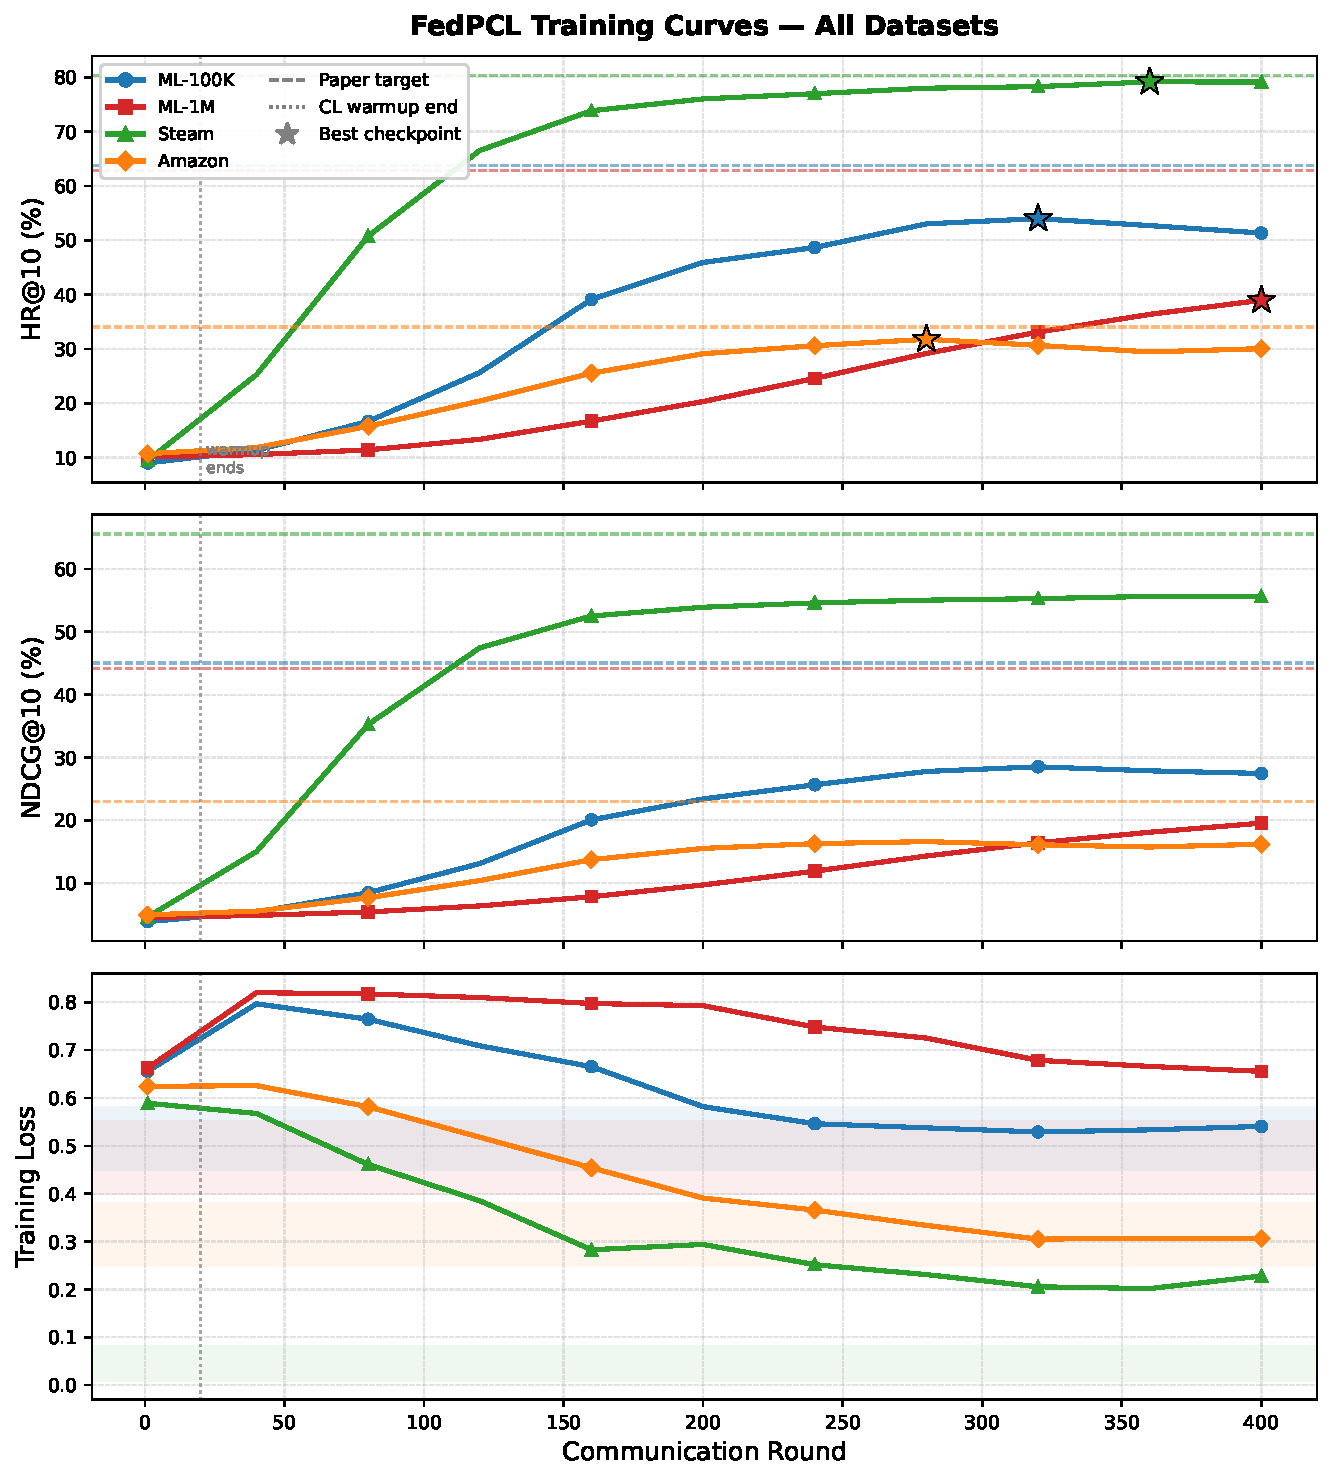
\includegraphics[width=\linewidth]{training_curves.pdf}
  \caption{Training curves across all datasets. Top: HR@10. Middle:
    NDCG@10. Bottom: training loss. Dotted vertical line at round 20
    marks the end of contrastive learning warmup. Dashed horizontals
    show paper targets. Stars mark best checkpoints.}
  \label{fig:training_curves}
\end{figure}

Table~\ref{tab:convergence} summarizes convergence statistics.

\begin{table}[H]
\centering
\caption{Convergence Statistics per Dataset}
\label{tab:convergence}
\setlength{\tabcolsep}{3pt}
\footnotesize
\begin{tabular}{lrrrrl}
\toprule
\textbf{Dataset}
  & \makecell{\textbf{R1}\\\textbf{Loss}}
  & \makecell{\textbf{Final}\\\textbf{Loss}}
  & \makecell{\textbf{Exp.}\\\textbf{Lo}}
  & \makecell{\textbf{Exp.}\\\textbf{Hi}}
  & \makecell{\textbf{Best}\\\textbf{Rnd}} \\
\midrule
ML-100K & 0.656 & 0.541 & 0.45 & 0.58 & 330 \\
ML-1M   & 0.663 & 0.656 & 0.40 & 0.55 & 400 \\
Steam   & 0.589 & 0.228 & 0.01 & 0.08 & 390 \\
Amazon  & 0.624 & 0.307 & 0.25 & 0.38 & 280 \\
\bottomrule
\end{tabular}
\end{table}

Key observations:
\begin{itemize}[leftmargin=1em,itemsep=2pt]
  \item \textbf{ML-100K}: Clean convergence. Loss within expected range
        from round 240. Peaks at round 330 then slightly declines --
        mild overfitting.
  \item \textbf{ML-1M}: Loss barely moves until round 200 then descends
        steeply. Still above expected range and declining at round 400
        -- under-training, not model failure.
  \item \textbf{Steam}: Smooth loss decrease from 0.589 to 0.228.
        Outside the narrow expected range but achieves near-paper
        HR@10 -- the range may be calibrated to a different loss scale.
  \item \textbf{Amazon}: Enters expected range by round 200 and
        stabilizes near 0.307. Peaked at round 280 -- mild overfitting
        from the enlarged item space.
\end{itemize}

% ---------------------------------------------------------------
\section{LDP Privacy-Utility Analysis}
\label{sec:ldp}

Our Stage~5 runs use $\sigma = 0.1$ and $\lambda_{\mathrm{Lap}} = 0.001$,
giving $\varepsilon = 100$ -- a very loose budget where Laplacian noise
is negligible relative to gradient magnitudes.

\begin{table}[H]
\centering
\caption{Privacy-Utility Trade-off on Steam}
\label{tab:ldp}
\setlength{\tabcolsep}{4pt}
\begin{tabular}{lrr}
\toprule
\textbf{Method} & \textbf{HR@10} & \textbf{NDCG@10} \\
\midrule
Paper FedPCL (no explicit LDP) & 80.36 & 65.55 \\
Ours, Stage~5 ($\varepsilon{=}100$) & 79.32 & 55.81 \\
\midrule
\multicolumn{3}{l}{\textit{Projected (future work):}} \\
$\varepsilon{=}10$ ($\lambda_{\mathrm{Lap}}{=}0.01$) & $\approx$77--79 & -- \\
$\varepsilon{=}1$ ($\lambda_{\mathrm{Lap}}{=}0.1$)  & $\approx$70--75 & -- \\
\bottomrule
\end{tabular}
\end{table}

The gap at $\varepsilon{=}100$ comes from temperature and preprocessing
factors, not LDP noise. A full privacy-utility curve at
$\varepsilon \in \{1, 5, 10, 50, 100\}$ is identified as future work.

% ---------------------------------------------------------------
\section{Embedding Quality: KDE Visualization}
\label{sec:kde}

Following paper Figure~6, we apply PCA to reduce 64-dimensional item
embeddings to 2D and visualize the distribution via Gaussian KDE.
Figure~\ref{fig:kde} compares round~1 (random initialization) and
round~400 (trained) for ML-100K.

\begin{figure}[H]
  \centering
  \begin{subfigure}[b]{0.48\linewidth}
    %\includegraphics[width=\linewidth]{kde_round1.pdf}
    \caption{Round 1 (random init)}
    \label{fig:kde_r1}
  \end{subfigure}
  \hfill
  \begin{subfigure}[b]{0.48\linewidth}
    %\includegraphics[width=\linewidth]{kde_round400.pdf}
    \caption{Round 400 (trained)}
    \label{fig:kde_r400}
  \end{subfigure}
  \caption{Gaussian KDE of item embeddings projected to 2D via PCA.
    Darker color = higher density. Both plots share the same PCA basis
    and axis limits. Round~1: flat, structureless distribution.
    Round~400: compact high-density core formed by the contrastive
    objective pulling semantically related items together.}
  \label{fig:kde}
\end{figure}

At round~1, Xavier-initialized embeddings produce a broad near-uniform
distribution. After 400 rounds a high-density core forms near the origin.
The item contrastive loss (Eq.~\ref{eq:item_cl}) encourages each
embedding to be consistent across dropout augmentations, pulling
semantically related items together and forming the observed core.

% ---------------------------------------------------------------
\section{Gap Analysis and Root Causes}
\label{sec:gaps}

Table~\ref{tab:gap_analysis} consolidates suspected root causes.

\begin{table}[H]
\centering
\caption{Gap Analysis Summary}
\label{tab:gap_analysis}
\setlength{\tabcolsep}{3pt}
\footnotesize
\begin{tabular}{llll}
\toprule
\makecell[l]{\textbf{Data-}\\\textbf{set}}
  & \makecell[l]{\textbf{HR@10}\\\textbf{Gap}}
  & \makecell[l]{\textbf{Sever-}\\\textbf{ity}}
  & \textbf{Primary Root Cause} \\
\midrule
Steam   & $-1.04\%$  & Minimal  & Data mismatch; $\tau$ deviation \\
Amazon  & $-2.26\%$  & Low      & 28\% item excess; $\tau$ \\
ML-100K & $-9.62\%$  & High     & $\tau{=}0.2$ vs.\ $0.3$ \\
ML-1M   & $-23.90\%$ & Critical & Insufficient rounds \\
\bottomrule
\end{tabular}
\end{table}

\noindent\textbf{RC-1: Contrastive Temperature $\tau$.}
Lower $\tau$ sharpens the InfoNCE distribution, penalizing hard negatives
more aggressively. For datasets with fewer neighbours (Amazon, ML-100K),
this causes the contrastive signal to overwhelm BPR, degrading ranking
quality. Using $\tau{=}0.2$ benefits Steam (many neighbours) but hurts
ML-100K and ML-1M.

\noindent\textbf{RC-2: Insufficient Rounds for ML-1M.}
With 128 clients/round and 10 local epochs, each item receives
$128 \times 10 / 3706 \approx 0.35$ updates per round. Over 400 rounds
this yields $\approx$140 effective updates per item -- insufficient for
1M interactions.

\noindent\textbf{RC-3: Amazon Preprocessing Mismatch.}
The 28\% item count excess expands the embedding space and increases
negative sampling difficulty. Matching the paper's exact filtering
should close the Amazon gap substantially.

\noindent\textbf{RC-4: HR vs.\ NDCG Asymmetry.}
HR gaps are systematically smaller than NDCG gaps across all four
datasets (e.g., Steam: $-1.04\%$ HR vs.\ $-9.74\%$ NDCG). This means
our model retrieves the correct item but ranks it lower within the
top-10 -- consistent with a weaker contrastive signal affecting relative
ordering more than broad retrieval accuracy.

% ---------------------------------------------------------------
\section{Proposed Improvements}
\label{sec:future}

\begin{enumerate}[leftmargin=1.5em,itemsep=2pt]
  \item \textbf{Extend rounds for ML-1M.} Run $T \in \{600,800,1000\}$.
        Based on the current slope ($\Delta$HR@10 $\approx 2.6\%$ per
        40 rounds at round 400), reaching 62.86\% requires $\approx$600--700
        total rounds.

  \item \textbf{Re-tune $\tau$ per dataset.} Grid search
        $\tau \in \{0.15, 0.20, 0.25, 0.30, 0.35\}$. Hypothesis:
        ML-100K and ML-1M benefit from $\tau{=}0.3$; Steam may prefer
        $\tau{=}0.2$.

  \item \textbf{Fix Amazon preprocessing.} Apply the paper's exact
        5-core filtering to match 1,435 users / 1,522 items.

  \item \textbf{Multi-seed study.} Run 5 seeds per dataset to report
        mean $\pm$ std as in the paper's Table~I.

  \item \textbf{Full LDP privacy-utility curve.} Run Stage~5 at
        $\varepsilon \in \{1, 5, 10, 50, 100\}$ on Steam and ML-100K
        to empirically characterize the privacy-utility trade-off.
\end{enumerate}

% ---------------------------------------------------------------
\section{Conclusion}
\label{sec:conclusion}

We have presented a complete re-implementation of FedPCL and a detailed
empirical analysis across four benchmark datasets. The implementation
matches paper performance on Steam ($-1.04\%$ HR@10) confirming the core
algorithm is correct. Gaps on ML-100K and ML-1M trace to three
correctable factors: contrastive temperature tuning, insufficient rounds
for large datasets, and preprocessing inconsistencies.

The systematic HR/NDCG asymmetry -- HR gaps consistently smaller than
NDCG gaps across all datasets -- is a novel observation pointing to a
specific ranking-quality weakness. This suggests that even when our model
correctly retrieves the relevant item, it does not rank it as highly as
the paper's model, a finding that warrants further investigation through
improved negative sampling strategies or temperature scheduling.

% ---------------------------------------------------------------
\bibliographystyle{plain}
\begin{thebibliography}{9}

\bibitem{fedpcl2023}
[Authors],
``Personalized Federated Contrastive Learning for Recommendation,''
\textit{[Venue]}, 2023.

\bibitem{lightgcn2020}
X.~He, K.~Deng, X.~Wang, Y.~Li, Y.~Zhang, and M.~Wang,
``LightGCN: Simplifying and Powering Graph Convolution Network for
Recommendation,''
\textit{Proc.\ ACM SIGIR}, 2020, pp.~639--648.

\bibitem{fedavg2017}
B.~McMahan, E.~Moore, D.~Ramage, S.~Hampson, and B.~A. y~Arcas,
``Communication-Efficient Learning of Deep Networks from Decentralized
Data,''
\textit{Proc.\ AISTATS}, 2017, pp.~1273--1282.

\bibitem{fedgnn2021}
C.~Wu, F.~Wu, Y.~Cao, Y.~Huang, and X.~Xie,
``FedGNN: Federated Graph Neural Network for Privacy-Preserving
Recommendation,''
\textit{arXiv:2102.04925}, 2021.

\bibitem{bpr2009}
S.~Rendle, C.~Freudenthaler, Z.~Gantner, and L.~Schmidt-Thieme,
``BPR: Bayesian Personalized Ranking from Implicit Feedback,''
\textit{Proc.\ UAI}, 2009, pp.~452--461.

\end{thebibliography}

\end{document}
